\section{Summary of Data Sets}\label{sec:data-summary}

In \Cref{tab:dataset-info} we summarize the data sets we use in our paper. Here, we also
provide brief descriptions of what these data sets represent.

\paragraph{a1a}

The a1a dataset is a binary classification dataset featuring 1605 observations and 123
binary features. This is a subset of the Adult dataset~\citep{becker1996,platt1998}
derived from census data, where the task is to predict whether a person's income exceeds
USD~50,000 per year based on census information.

\paragraph{w1a}

The w1a dataset is a binary classification dataset containing 2477 samples and 300 binary
features. It is derived from web page data, where each instance represents a web page and
the classification task is to determine whether the page belongs to a specific
category~\citep{platt1998}.

\paragraph{rhee2006}

The rhee2006 dataset contains 842 samples with 361 binary features and a continuous
response variable. It is derived from HIV-1 drug resistance research by \citet{rhee2006}
, where features represent HIV-1 protease and reverse transcriptase mutations, and the
response variable measures in vitro susceptibility to antiretroviral drugs. The dataset was
used to identify genotype-phenotype associations relevant to understanding drug resistance
patterns.

\paragraph{housing}

This is the classical Boston housing dataset~\citep{harrison1978}, which consists of
506 instances with 13 mixed-type features (including one binary feature) and a continuous
response variable. It contains information about housing in the Boston area, where the
response is the median value of owner-occupied homes in USD 1000s.

\paragraph{leukemia}

The leukemia dataset is a high-dimensional dataset with only 38 samples but 7129 continuous
features, with a binary response variable. It represents gene expression data for leukemia
patients~\citep{golub1999}, where the classification task is to distinguish between
acute myeloid leukemia (AML) and acute lymphoblastic leukemia (ALL) based on gene
expression profiles. This dataset was used to demonstrate the feasibility of cancer
classification based solely on gene expression monitoring.

\paragraph{triazines}

The triazines dataset contains 186 samples with 60 mixed-type features and a continuous
response variable. It is a pharmaceutical dataset relating the molecular structures of
2,4-diamino-6,6-dimethyl-5-phenyl-dihydrotriazine derivatives to their ability to inhibit
dihydrofolate reductase (DHFR)~\citep{hirst1994,king1995}. This dataset has been widely
used to develop quantitative structure-activity relationships (QSAR) and compare different
machine learning methods for predicting biological activity based on molecular structure.

\begin{table}
  \centering
  \caption{Details of the real datasets used in the experiments, The median \(q\) value
    refers to the median of the proportion of ones for the binary features in the data. Note that in the case of \data{housing}, there is
    only a single binary feature.}
  \label{tab:dataset-info}
  \begin{tabular}{
      l
      S[table-format=4.0]
      S[table-format=4.0]
      l
      l
      S[table-format=1.3,round-mode=places,round-precision=3]
    }
    \toprule
    Dataset   & {\(n\)} & {\(p\)} & Response   & Design     & {Median \(q\)} \\
    \midrule
    a1a       & 1605    & 123     & binary     & binary     & 0.970093       \\
    w1a       & 2477    & 300     & binary     & binary     & 0.976181       \\
    rhee2006  & 842     & 361     & continuous & binary     & 0.995249       \\
    housing   & 506     & 13      & continuous & mixed      & 0.93083        \\
    leukemia  & 38      & 7129    & binary     & continuous &                \\
    triazines & 186     & 60      & continuous & mixed      & 0.973118       \\
    \bottomrule
  \end{tabular}
\end{table}

We also visualize the distribution of class balance among all the binary features in
\Cref{fig:data-hist-q}. We note that the clas imbalance for these data sets is quite
severe, which is common for data sets, particularly in the high-dimensional regime.

\begin{figure}[htpb]
  \centering
  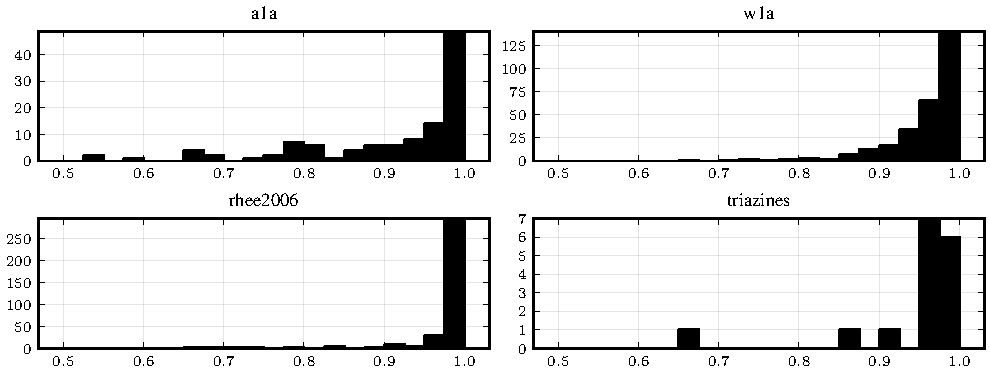
\includegraphics[]{data-hist-q.pdf}
  \caption{%
    Histograms over the distribution of \(q\) (class balance, that is, the
    proportion of ones) for the binary features in each of the data sets
    used in the paper.
  }
  \label{fig:data-hist-q}
\end{figure}

